\subsection{Stability analysis of explicit schemes}\label{sec:stability_explicit}
In figure~\ref{fig: ODEEXADERDeCeq}, we show the results obtained in \cite{Han_Veiga_2021}, extended up to order 13. It was pointed out, that the regions of the explicit ADER and DeC coincide and that they are independent of the chosen interpolation nodes. Here, we just display them once. We can highlight the growth of stability by increasing the order of the respective method. 
\begin{figure}[!h]
	\centering
	\begin{minipage}[t]{0.45\textwidth}
		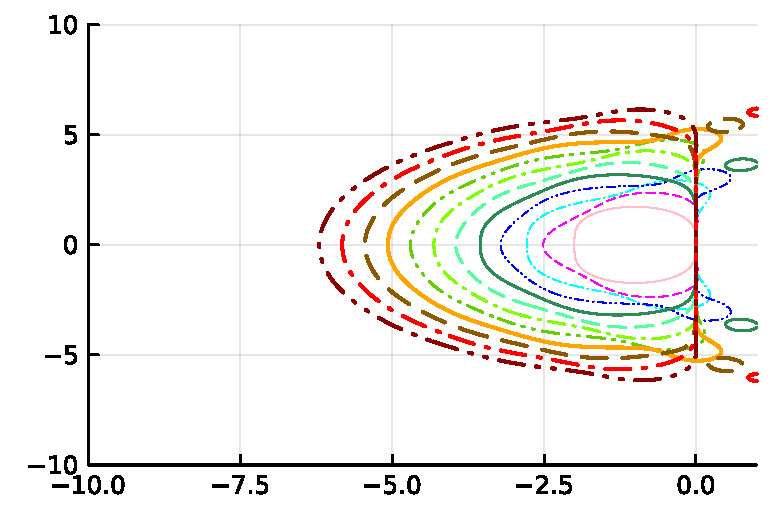
\includegraphics[width=\textwidth,trim={0 0 0 22}, clip]{pdf/odepics/DeC_GLB_ord13.pdf}
	\end{minipage}
	\caption{Stability regions for the explicit ADER and DeC methods with GLB or equispaced nodes for orders 2 to 13.}
	\label{fig: ODEEXADERDeCeq}
\end{figure}

Furthermore, we want to take a look at the explicit sDeC, whose stability regions can be observed in figure~\ref{fig: ODEEXsDeC}. 
This method differs not only from the ADER and DeC, but also from sDeC with different nodes. The qualitative shape is still similar to the others, but it is just remarkable that the sDeC methods with equispaced interpolation points have respectively larger stability regions.

\begin{figure}
	\centering
	\begin{minipage}[t]{0.45\textwidth}
		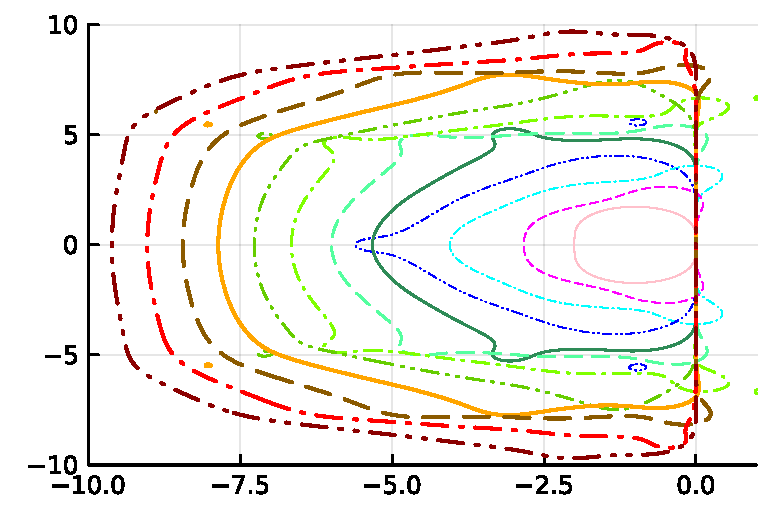
\includegraphics[width=\textwidth]{pdf/odepics/sDeC_eq_ord13.pdf}
	\end{minipage}
	\begin{minipage}[t]{0.45\textwidth}
		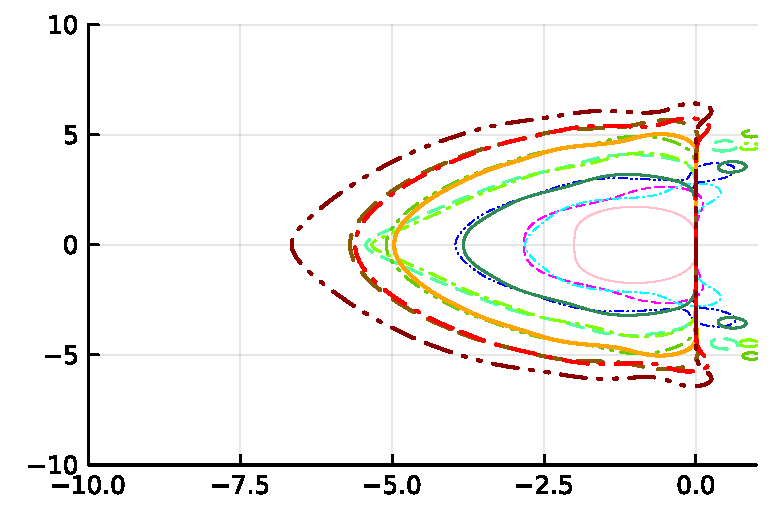
\includegraphics[width=\textwidth]{pdf/odepics/sDeC_GLB_ord13.pdf}
	\end{minipage}
	\caption{sDeC for orders 2 to 13.}
	\label{fig: ODEEXsDeC}
\end{figure}

%\subsection{The Robertson problem for explicit schemes}
%\label{subsec:robertson_explicit}
%The attempt to solve \eqref{eq: RobertsonODE} with the DeC6, sDeC6 and ADER6 with Gauss-Lobatto nodes for a different amount of time steps is shown figures \ref{fig: exaExRobertson_ord6_N=10^3} and \ref{fig: exaExRobertson_ord6_N=10^5}, where this behavior becomes recognizable. Increasing the time steps from $10^2$ to $10^5$ grants us just a few seconds of an accurate solution, before diverging to infinity rapidly, similarly to all other explicit methods.
%
%\begin{figure}
%	\centering
%	\begin{minipage}[t]{0.45\textwidth}
%		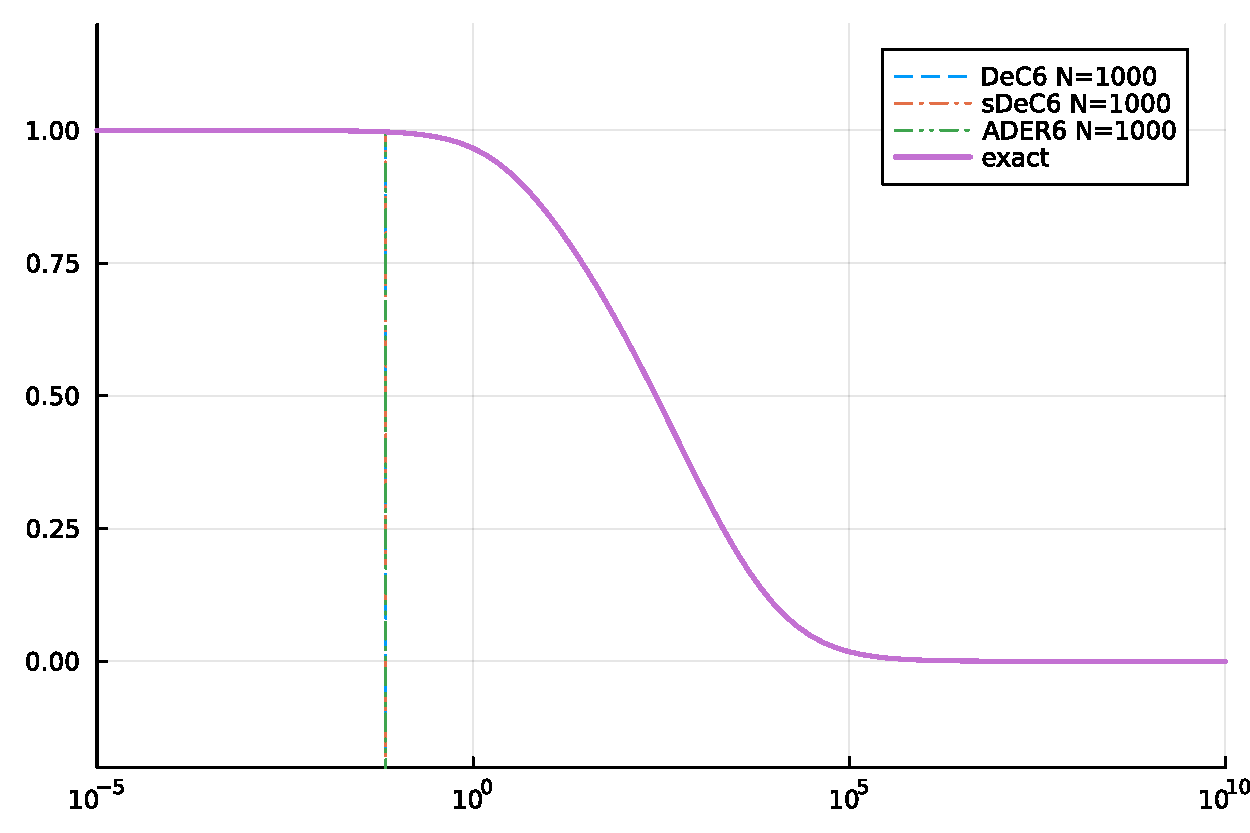
\includegraphics[width=\textwidth]{pdf/odepics/Num_val/EXrobertson_dim1_ord6_N=1000.pdf}
%	\end{minipage}
%	\begin{minipage}[t]{0.45\textwidth}
%		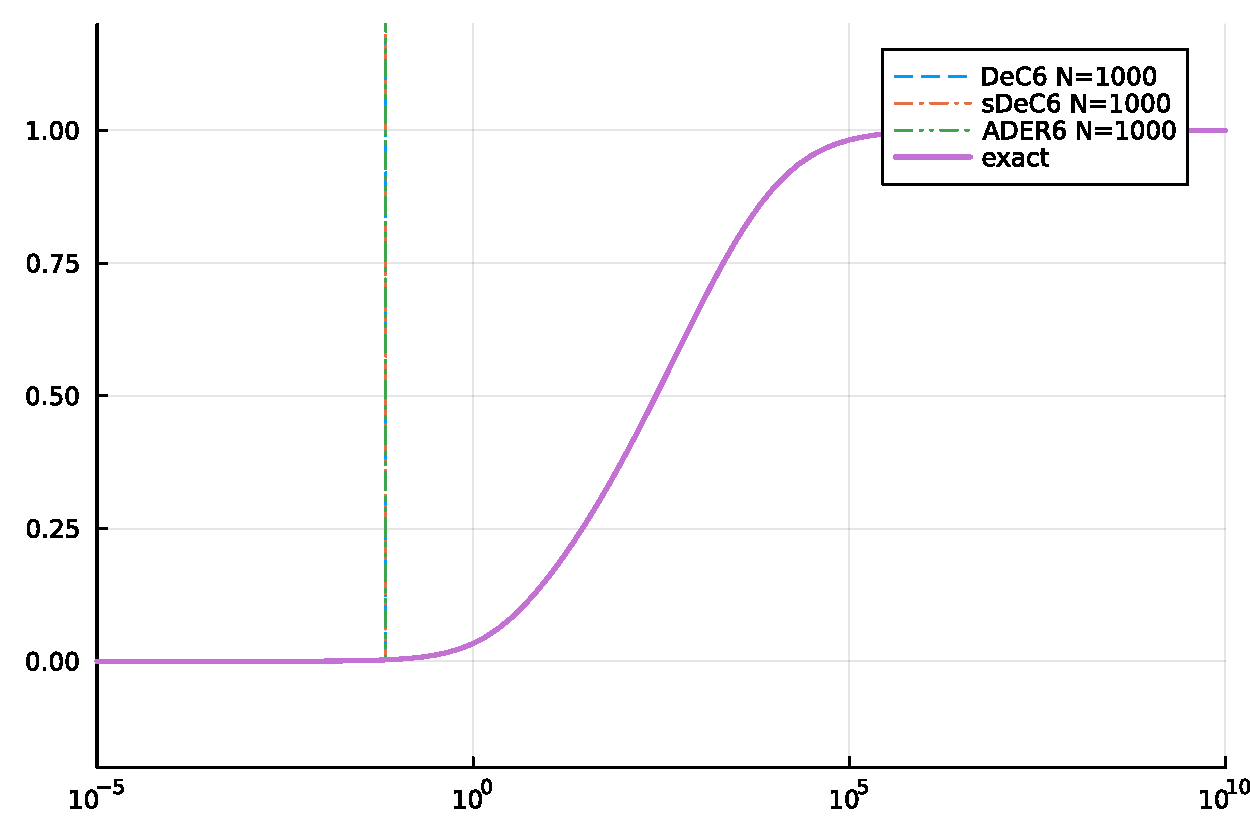
\includegraphics[width=\textwidth]{pdf/odepics/Num_val/EXrobertson_dim3_ord6_N=1000.pdf}
%	\end{minipage}
%	\caption{Solving equation \eqref{eq: RobertsonODE} using explicit methods of order 6 with GLB nodes for $u_1$ (left) and $u_3$ (right).}
%	\label{fig: exaExRobertson_ord6_N=10^3}
%\end{figure}
%
%\begin{figure}
%	\centering
%	\begin{minipage}[t]{0.45\textwidth}
%		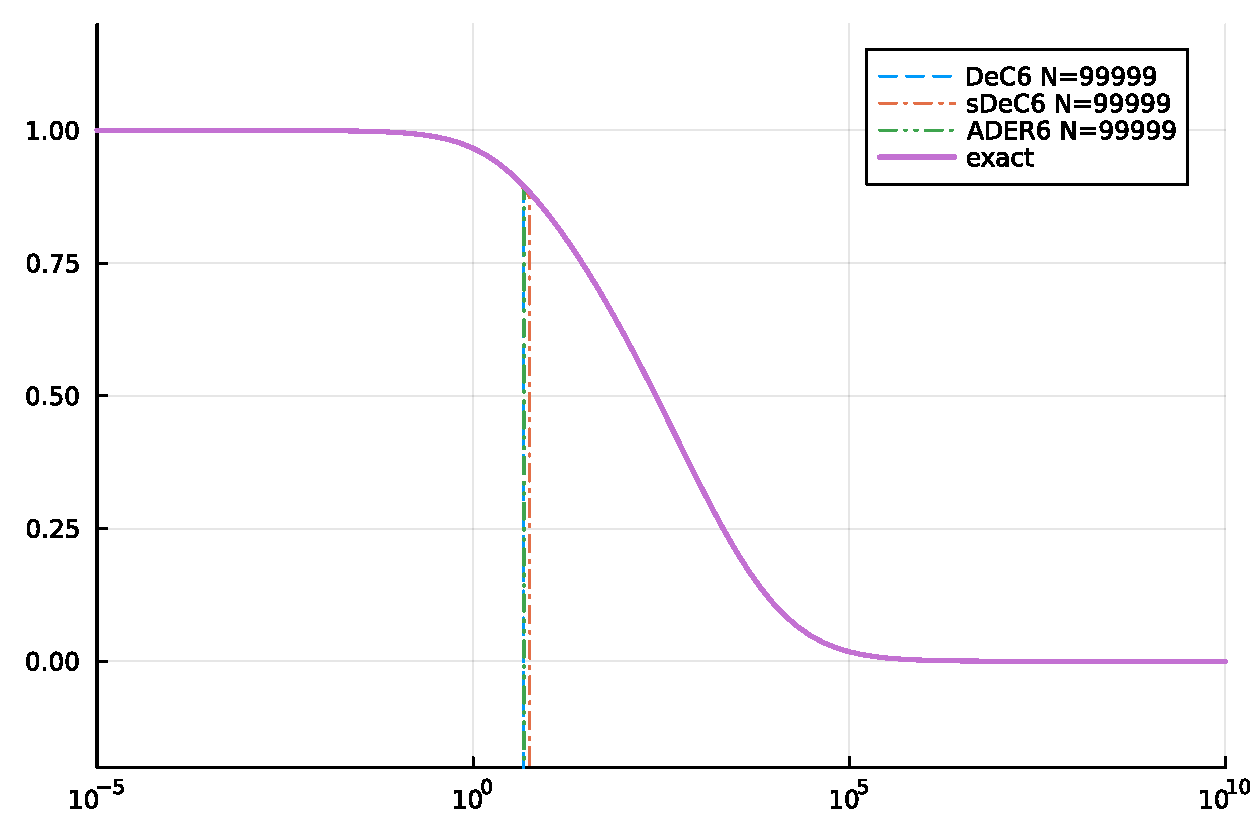
\includegraphics[width=\textwidth]{pdf/odepics/Num_val/EXrobertson_dim1_ord6_N=100000.pdf}
%	\end{minipage}
%	\begin{minipage}[t]{0.45\textwidth}
%		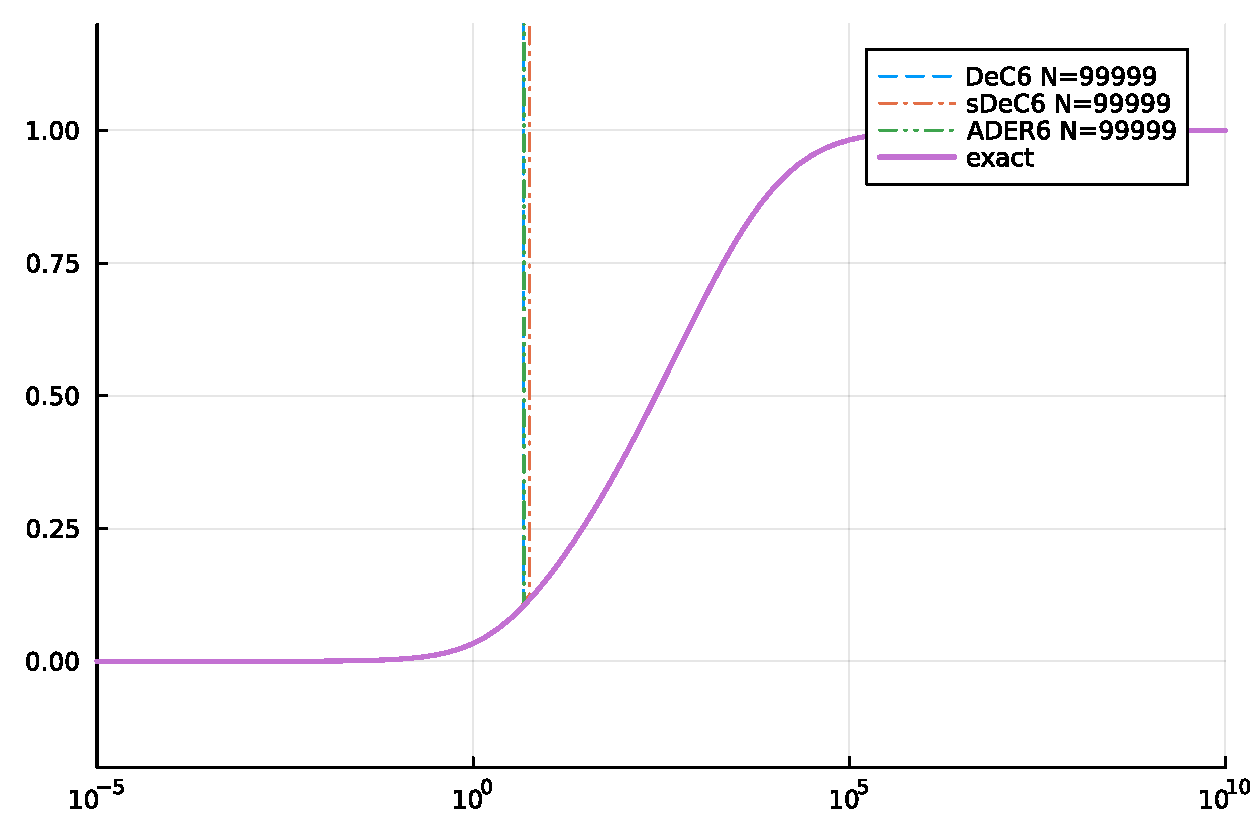
\includegraphics[width=\textwidth]{pdf/odepics/Num_val/EXrobertson_dim3_ord6_N=100000.pdf}
%	\end{minipage}
%	\caption{Solving equation \eqref{eq: RobertsonODE} using explicit methods of order 6 with GLB nodes for $u_1$ (left) and $u_3$ (right).}
%	\label{fig: exaExRobertson_ord6_N=10^5}
%\end{figure}